% !TEX root = ../../presentation.tex

\begin{slide}{Hardware: GPU}
  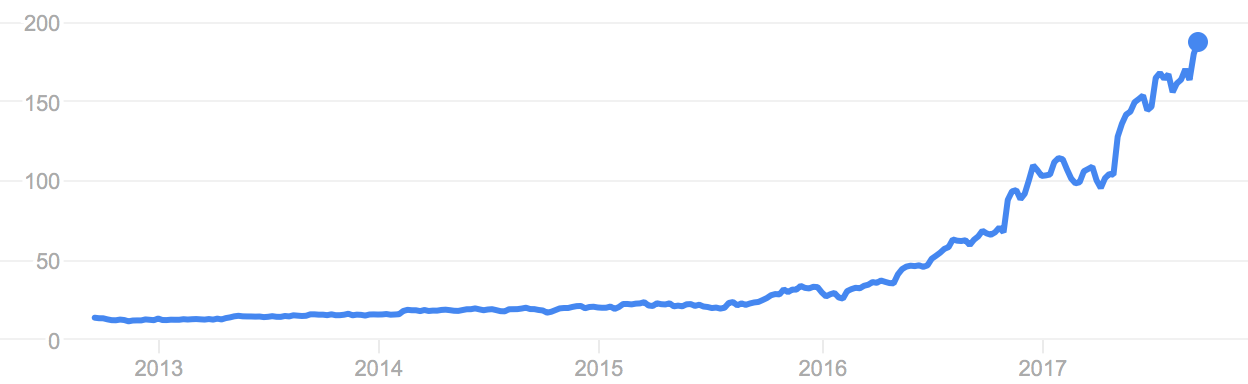
\includegraphics[width=8cm, height=2.75cm]{nvidia-stock}

  \textbf{NVIDIA Stock}

  \vspace{0.3cm}

  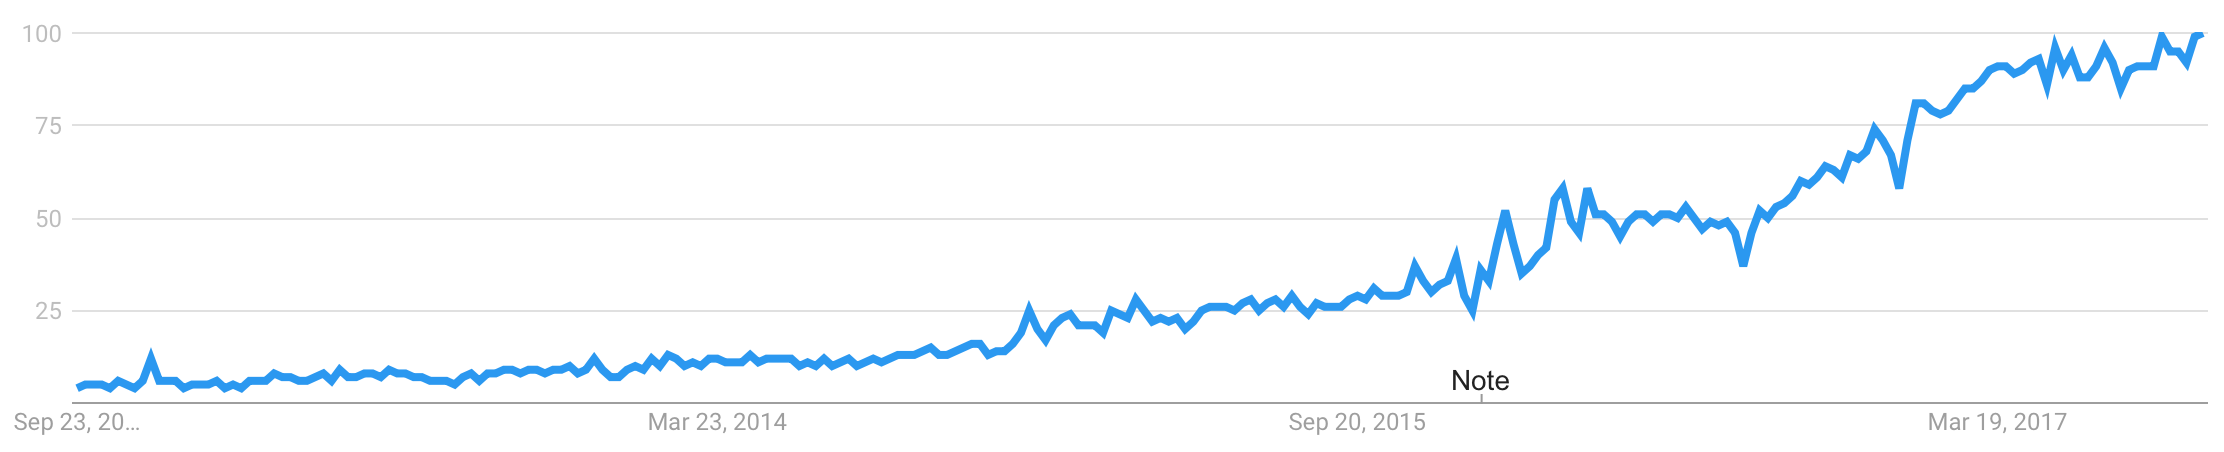
\includegraphics[width=8cm, height=2.75cm]{dl-trend}

  \textbf{Deep Learning Trend}
\end{slide}

\begin{slide}{Hardware: GPU}
  \begin{tikzpicture}
    \pause
    \node [inner sep=0] (titan) at (-3, 0)
          {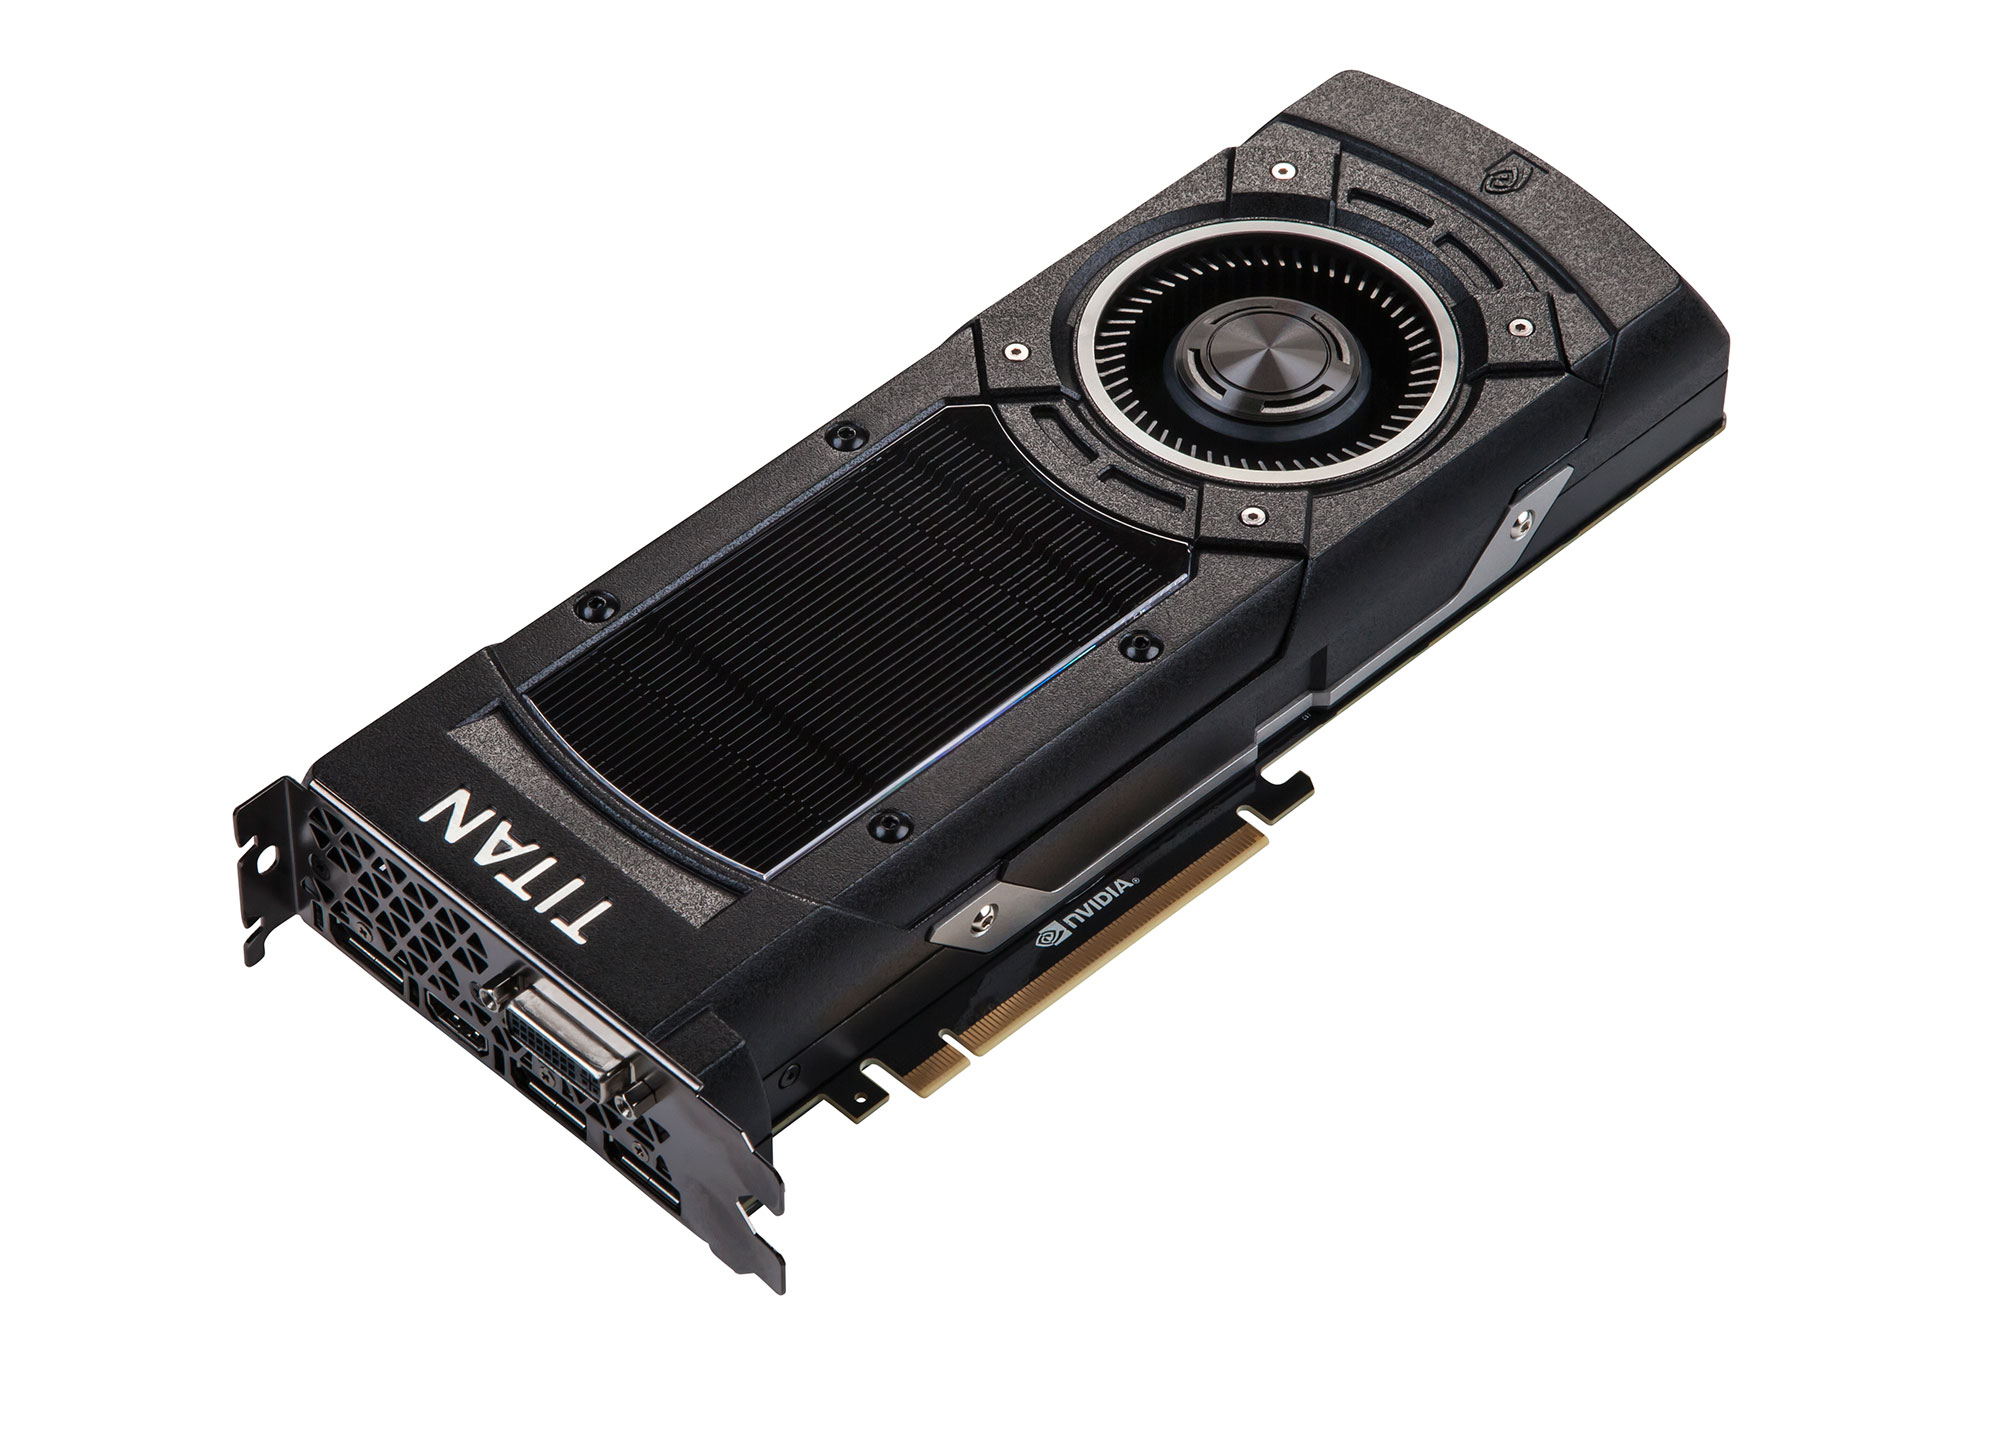
\includegraphics[width=4.5cm, height=2.7cm]{titan-x}};
    \draw [white, rounded corners=5pt, line width=5pt]
        (titan.north west) --
        (titan.north east) --
        (titan.south east) --
        (titan.south west) -- cycle;
    \draw (titan)+(0, -1.6) node {\textbf{Titan X}};

    \pause
    \node [inner sep=0] (tx2) at (+3, 0)
          {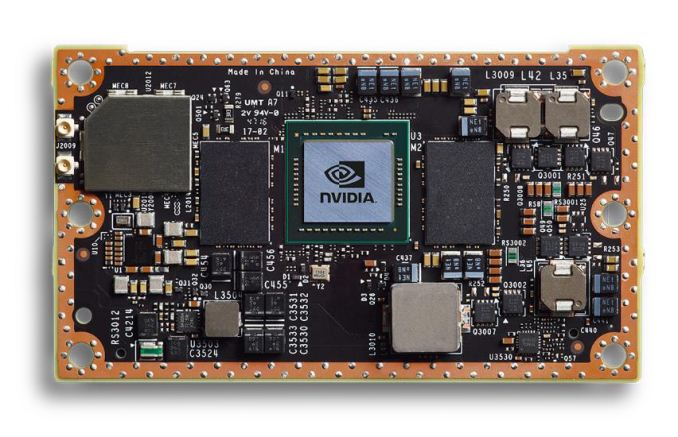
\includegraphics[width=4.5cm, height=2.7cm]{jetson-tx2}};
    \draw [white, rounded corners=5pt, line width=5pt]
        (tx2.north west) --
        (tx2.north east) --
        (tx2.south east) --
        (tx2.south west) -- cycle;
    \draw (tx2)+(0, -1.6) node {\textbf{Jetson TX2}};

    \pause
    \node [inner sep=0] (dgx1) at (0, -3.75)
          {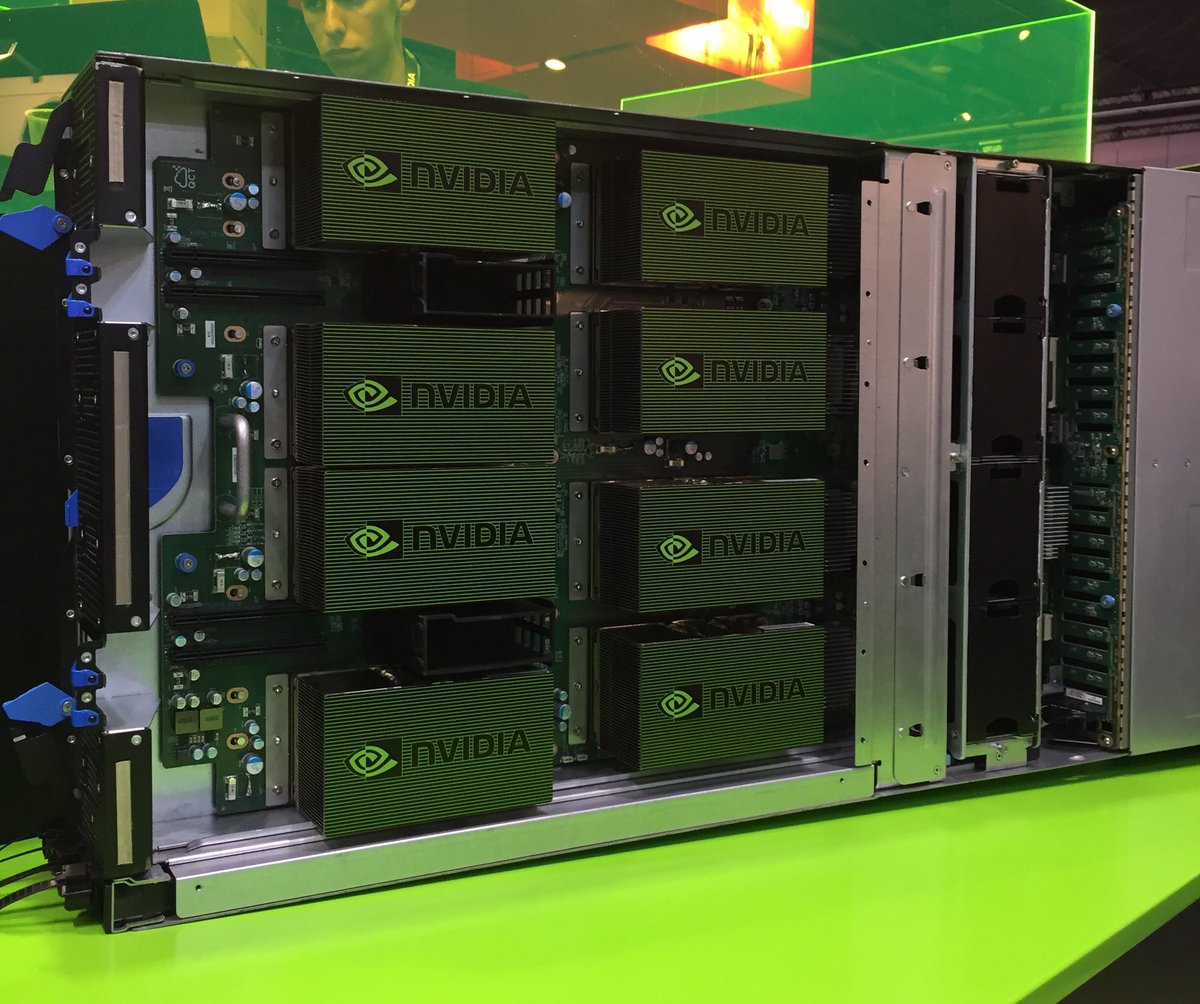
\includegraphics[width=4.5cm, height=3cm]{dgx-1}};
    \draw [white, rounded corners=5pt, line width=5pt]
        (dgx1.north west) --
        (dgx1.north east) --
        (dgx1.south east) --
        (dgx1.south west) -- cycle;
    \draw (dgx1)+(0, -1.8) node {\textbf{DGX-1}};
  \end{tikzpicture}
\end{slide}

% \begin{slide}{Hardware: Intel + Nervana}
%   \begin{tikzpicture}
%     \pause
%     \node [inner sep=0] (xeon) at (-3, 0)
%           {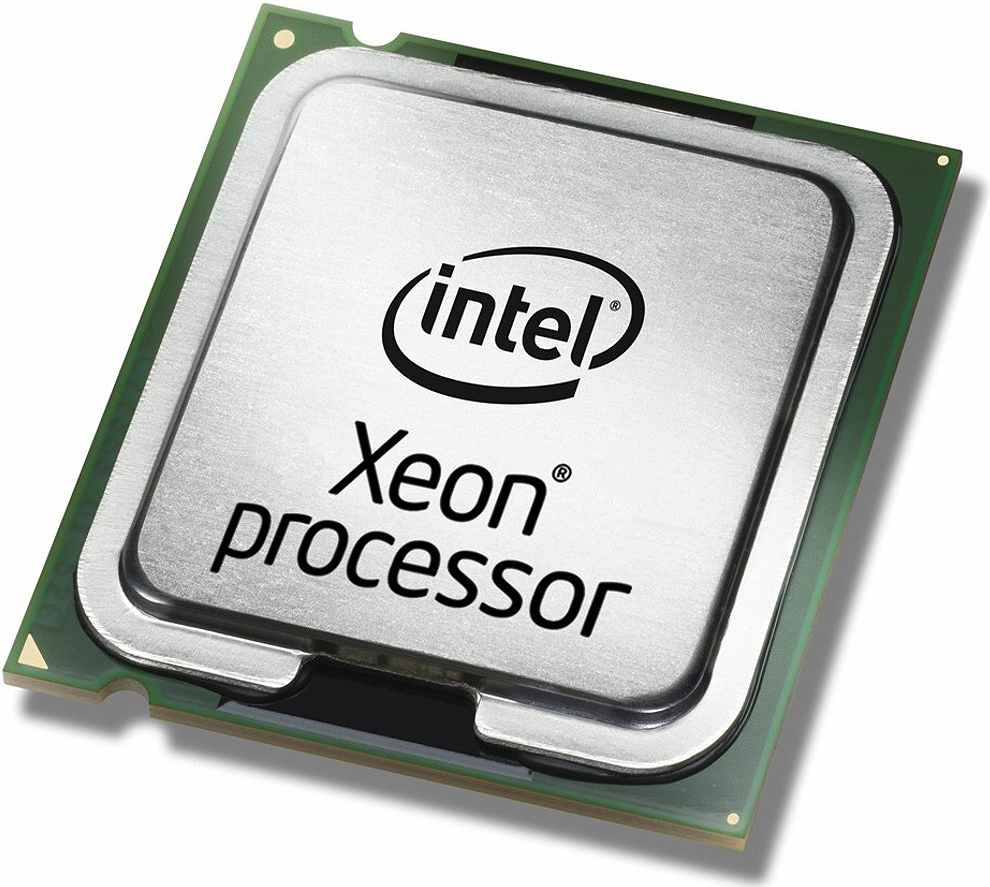
\includegraphics[width=4cm, height=2.2cm]{intel-xeon}};
%     \draw (xeon)+(0, -1.5) node {\textbf{Xeon}};
%
%     \pause
%     \node [inner sep=0] (mov) at (+3, 0)
%           {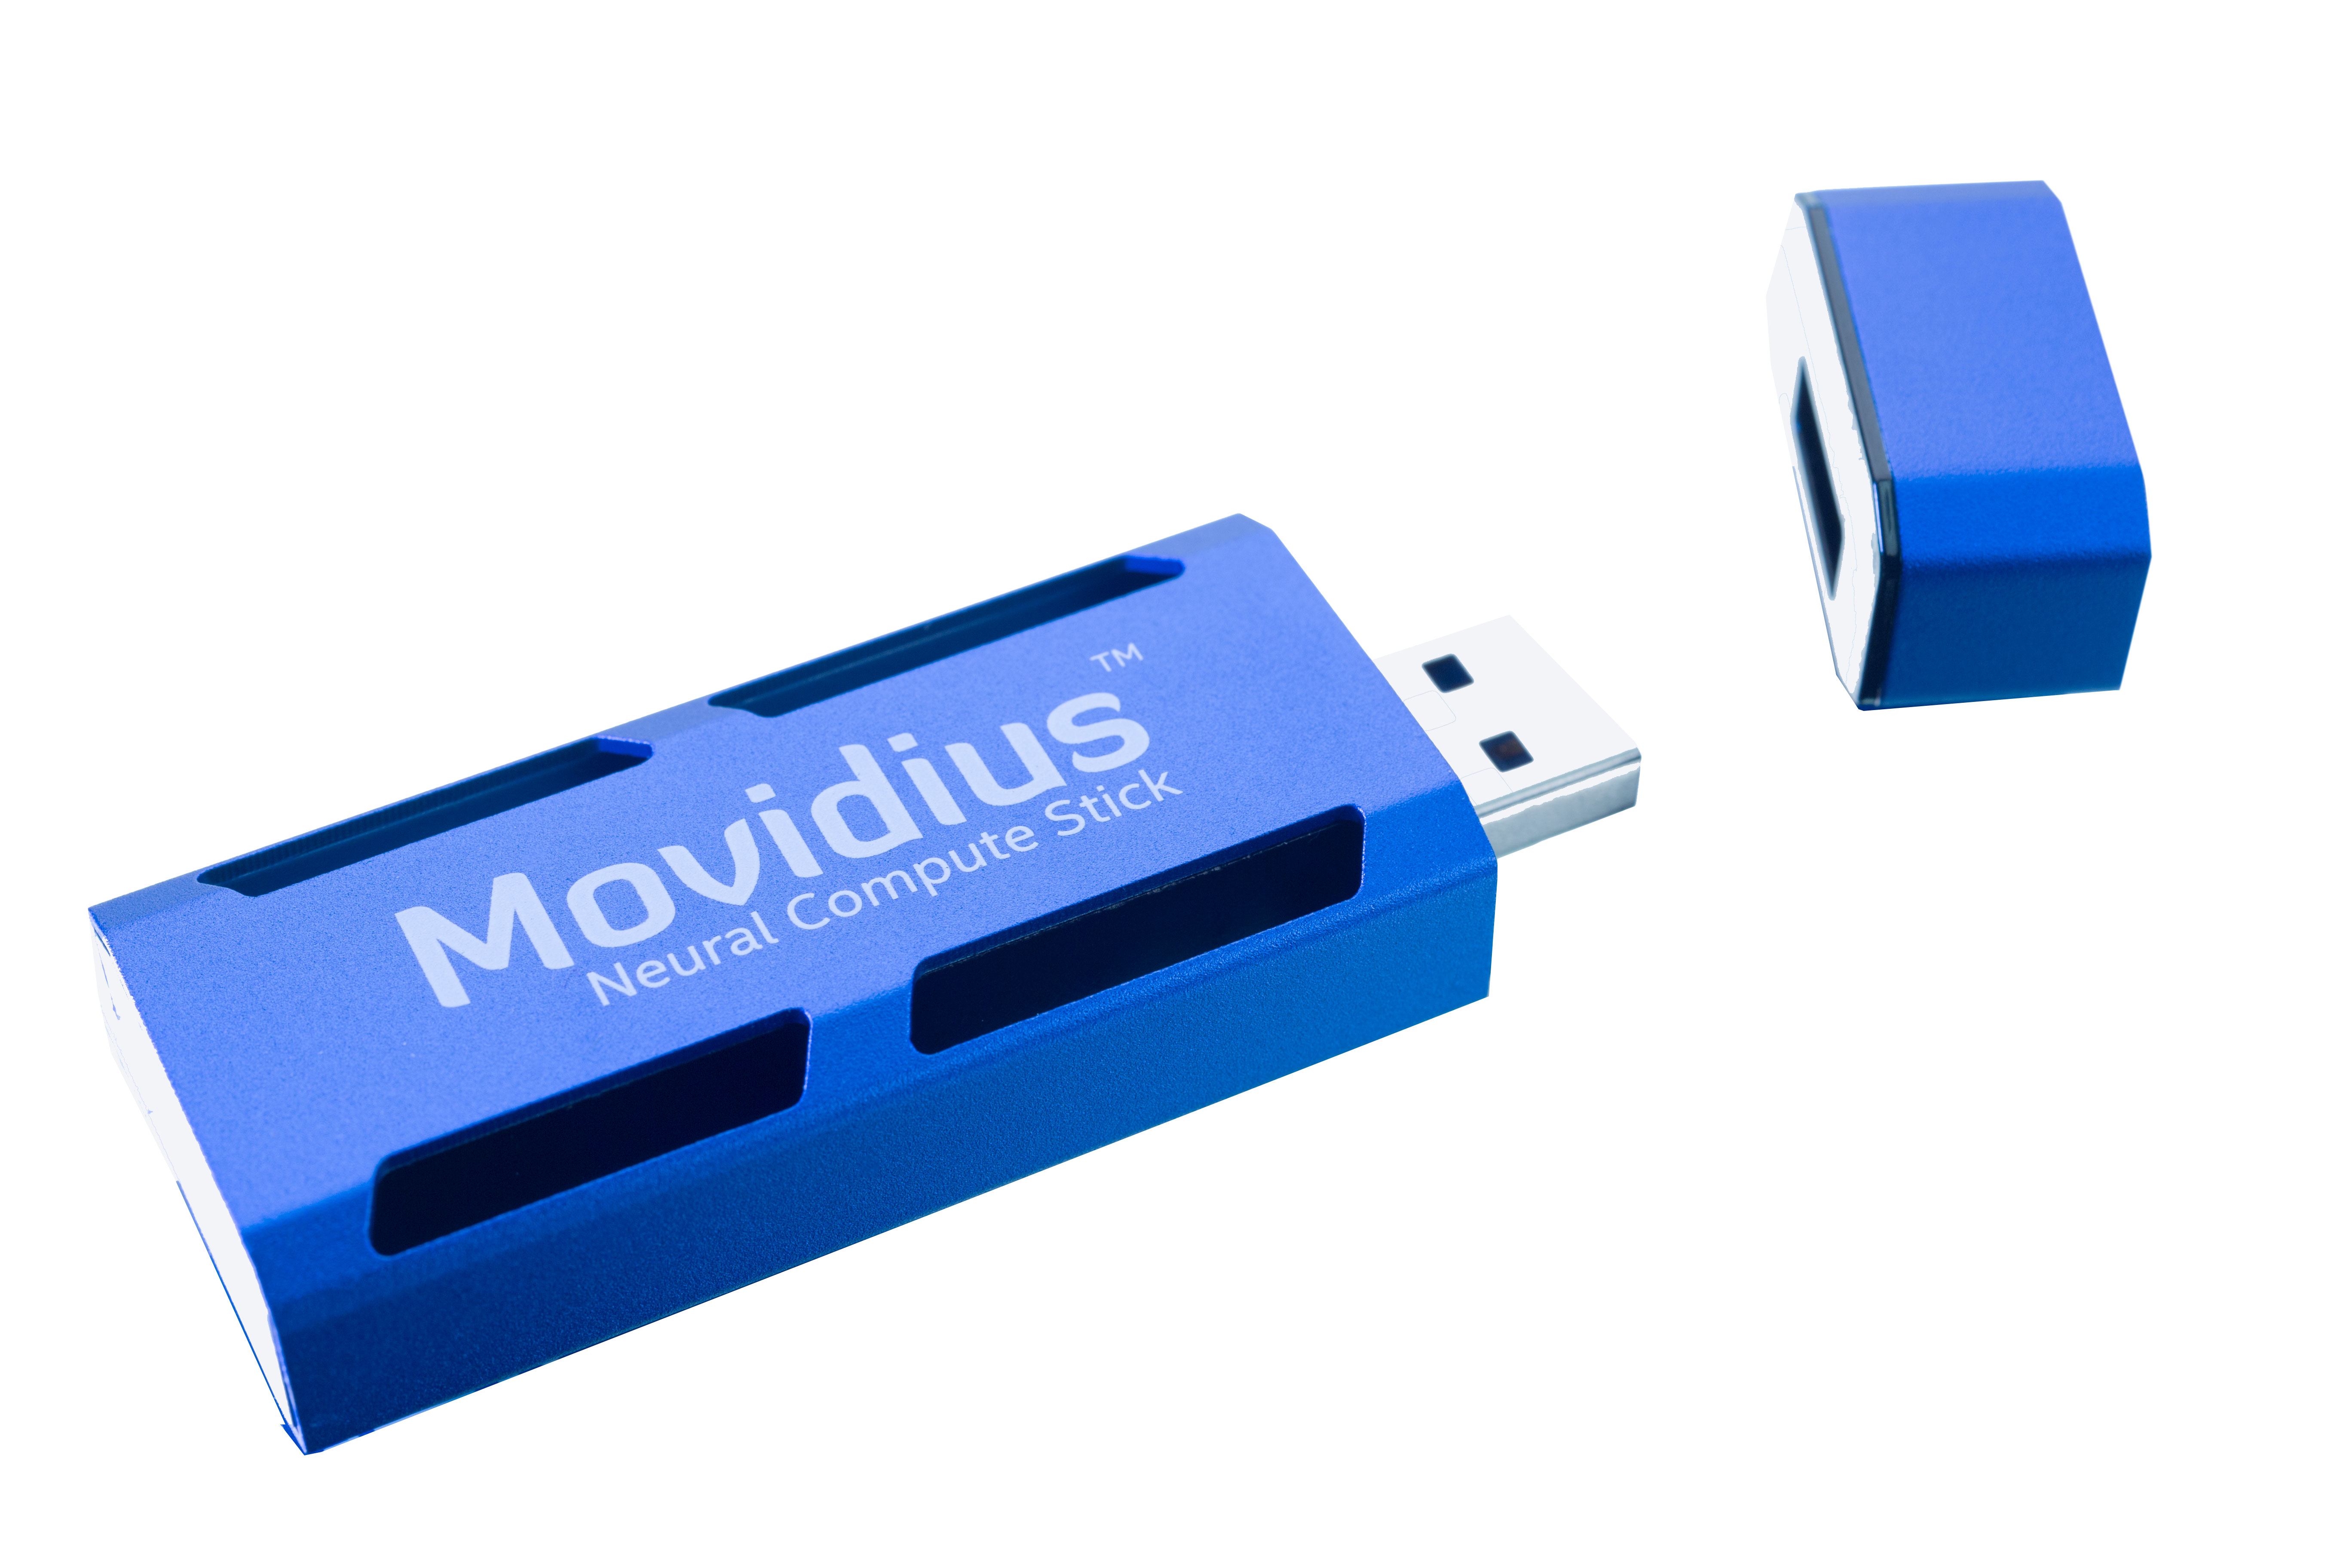
\includegraphics[width=4.5cm, height=2.7cm]{movidius}};
%     \draw (mov)+(0, -1.5) node {\textbf{Movidius VPU}};
%
%     \pause
%     \node [inner sep=0] (nervana) at (0, -3.7)
%           {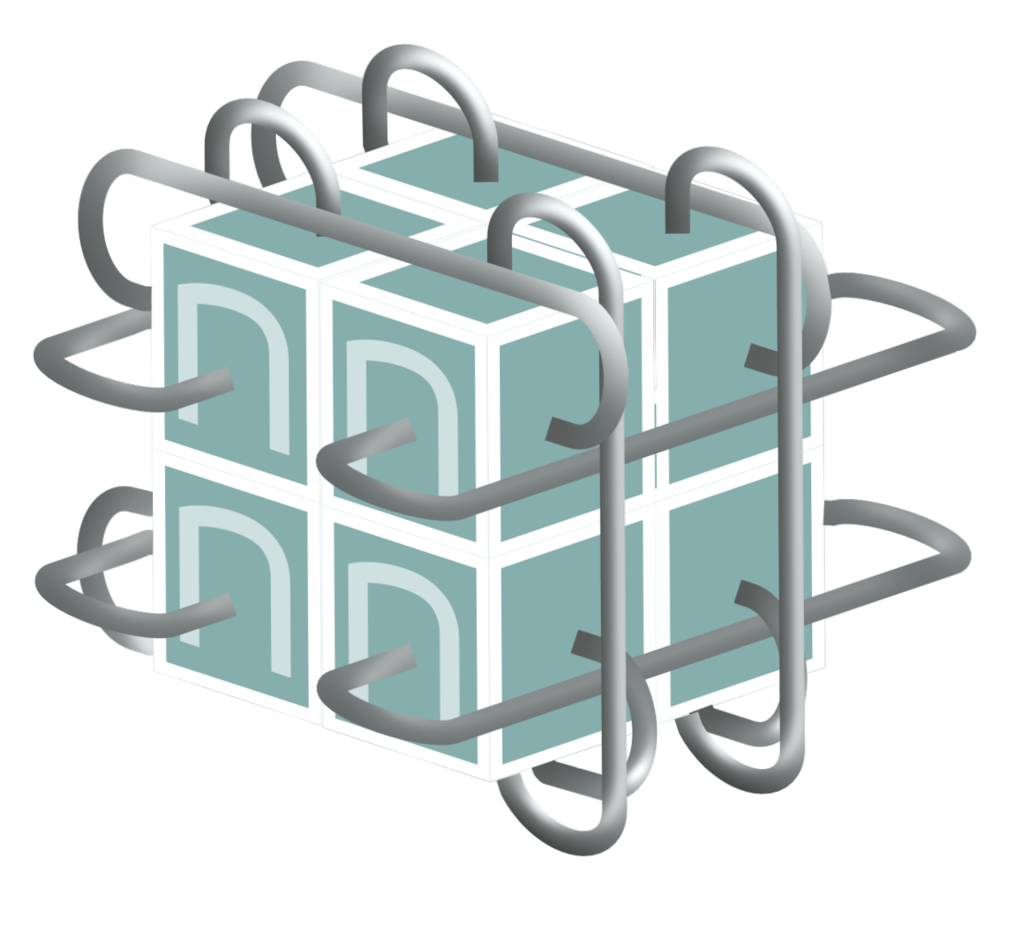
\includegraphics[width=4.5cm, height=4cm, trim={0 0 0 1.5cm}, clip]{nervana-engine}};
%     \draw (nervana)+(0, -2.1) node {\textbf{Nervana Engine}};
%   \end{tikzpicture}
% \end{slide}

\begin{slide}{Hardware: Big Basin}
  \begin{columns}
    \begin{column}{0.5\textwidth}
      \centering
      \begin{tikzpicture}
        \node [inner sep=0] (pic) at (0, 0)
              {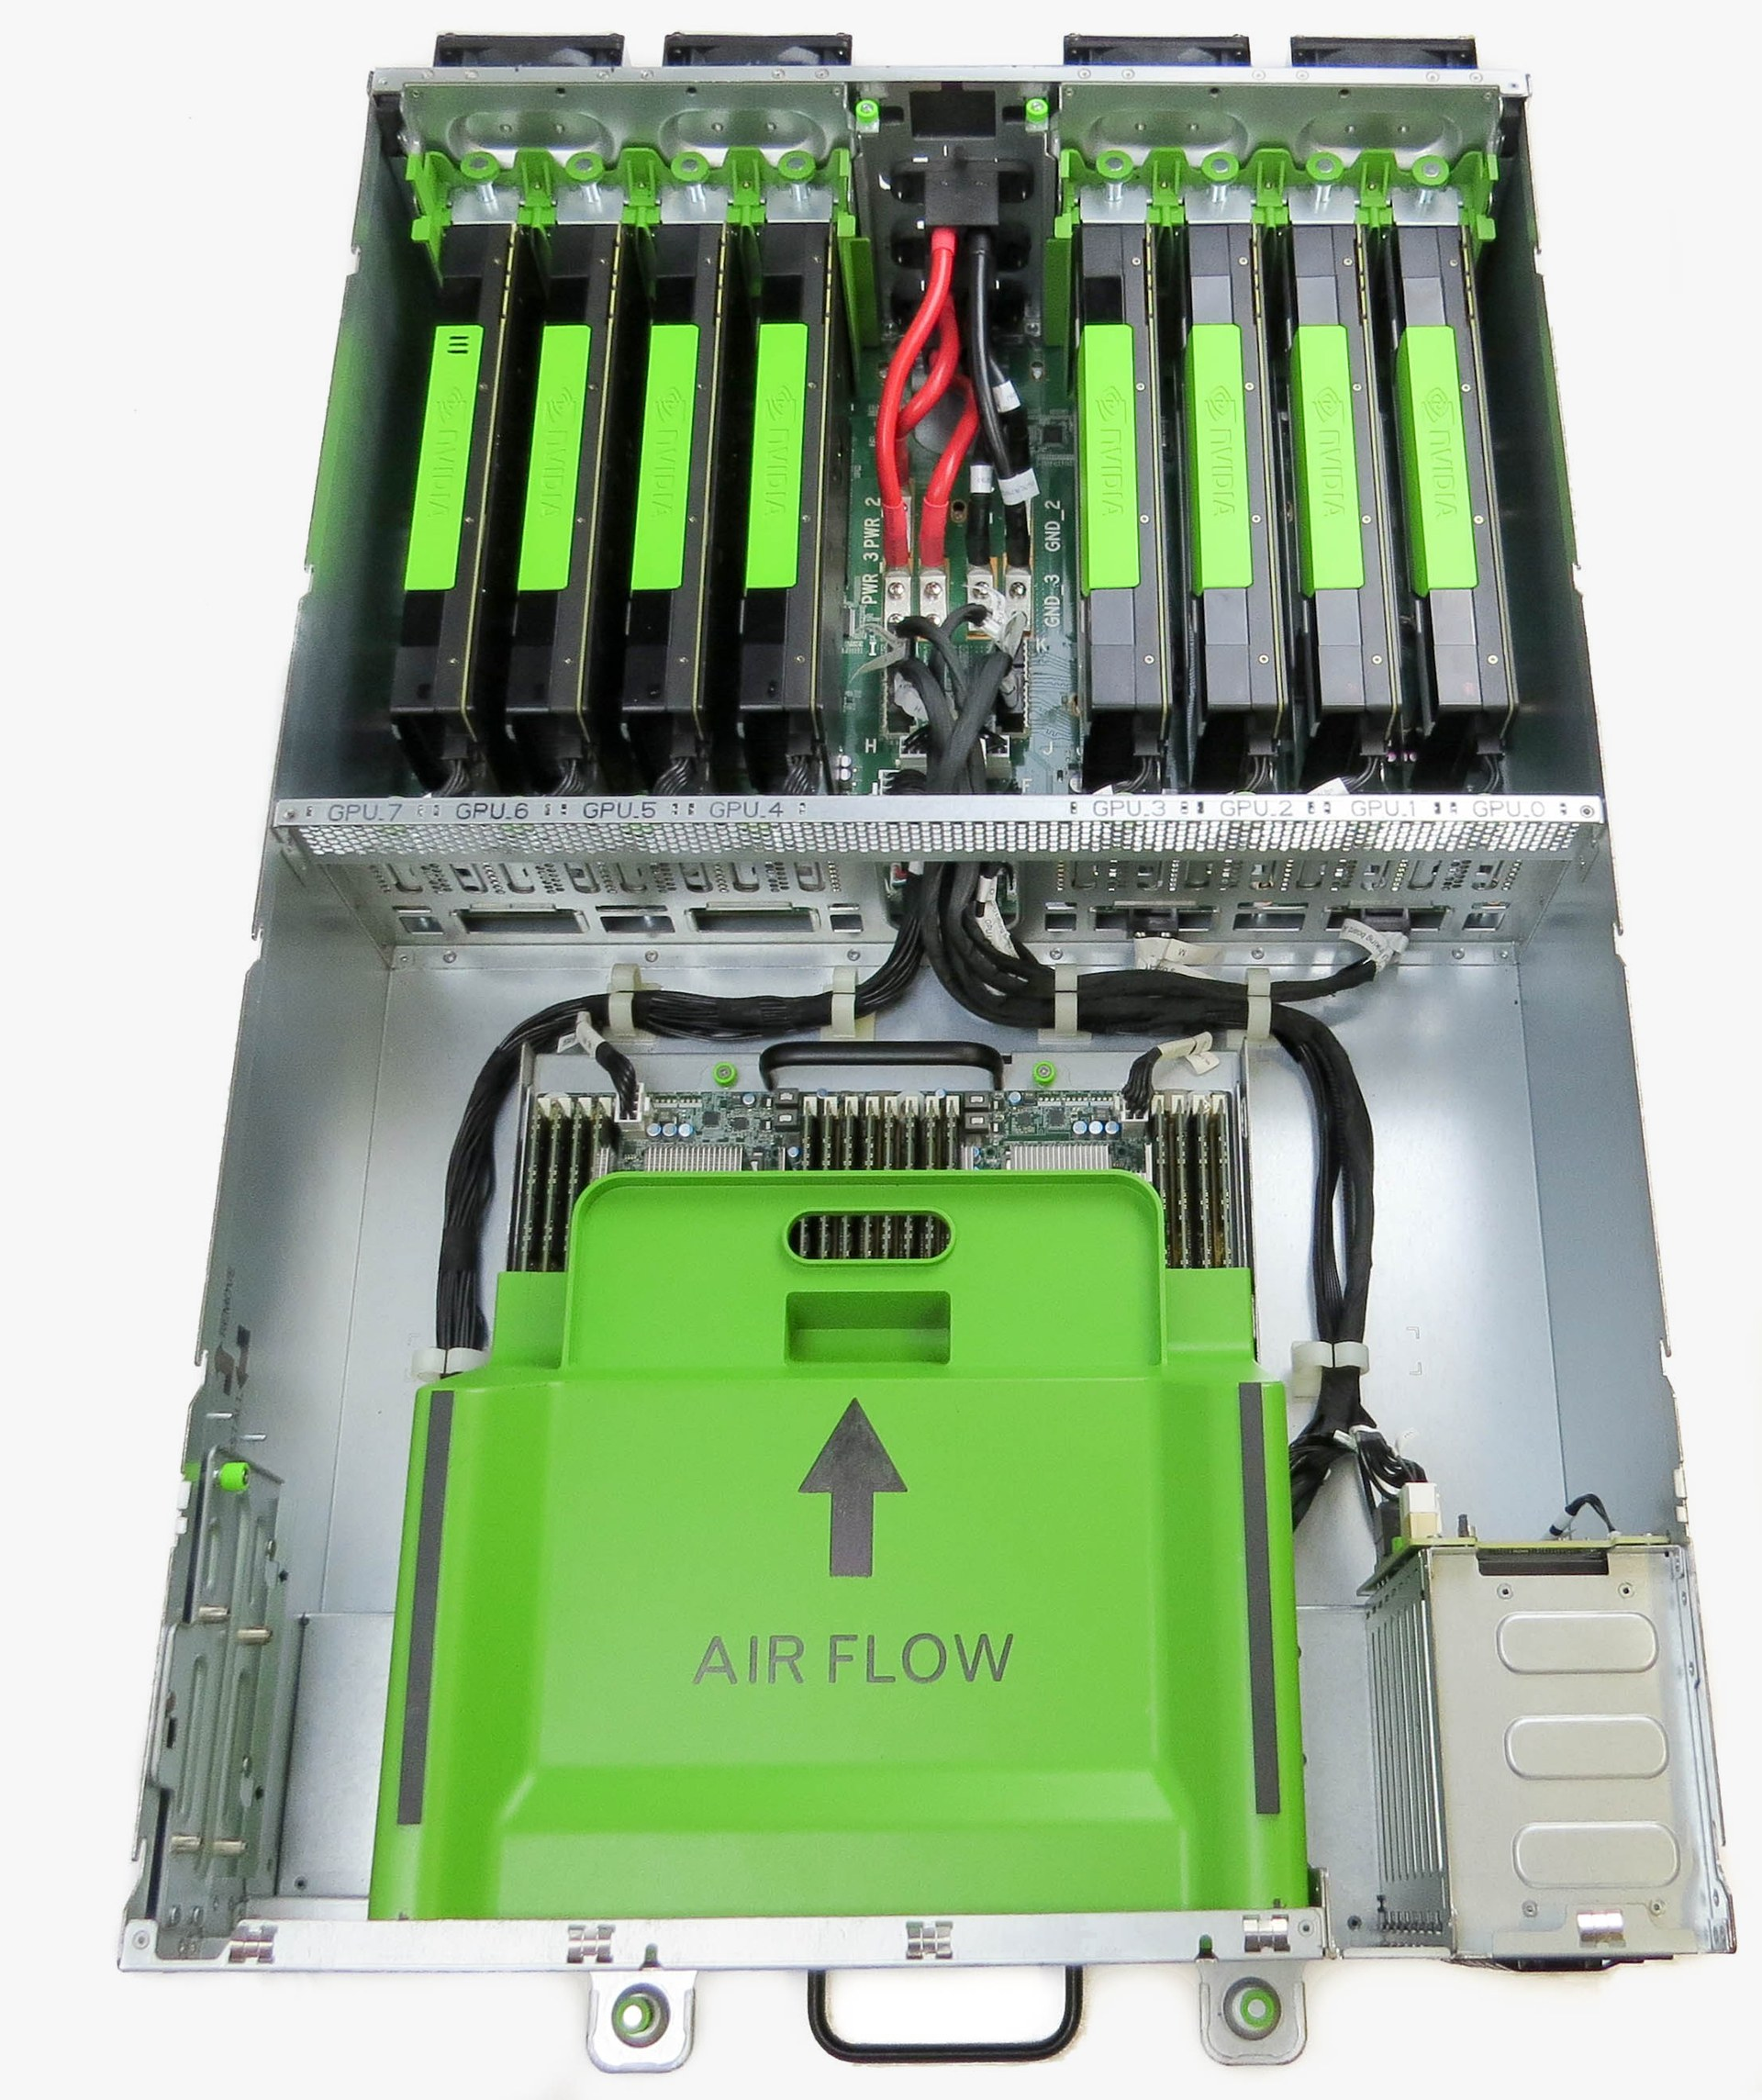
\includegraphics[scale=0.075]{big-sur}};
        \draw [white, rounded corners=5pt, line width=5pt]
            (pic.north west) --
            (pic.north east) --
            (pic.south east) --
            (pic.south west) -- cycle;
        \draw (pic)+(0, -3.4) node {\textbf{Big Basin}};
      \end{tikzpicture}
    \end{column}
    \begin{column}{0.55\textwidth}
      \begin{itemize}
        \item 8 NVIDIA Tesla P100 GPUs
        \item NVLink (12x faster than PCIe)
        \item 16 GB RAM
        \item 10.6 TFLOPS
        \item Reduced Precision Computing
      \end{itemize}
    \end{column}
  \end{columns}
\end{slide}

\begin{slide}{Hardware: TPU}
  \begin{columns}
    \begin{column}{0.55\textwidth}
      \centering
      \begin{tikzpicture}
        \node [inner sep=0] (pic) at (0, 0)
              {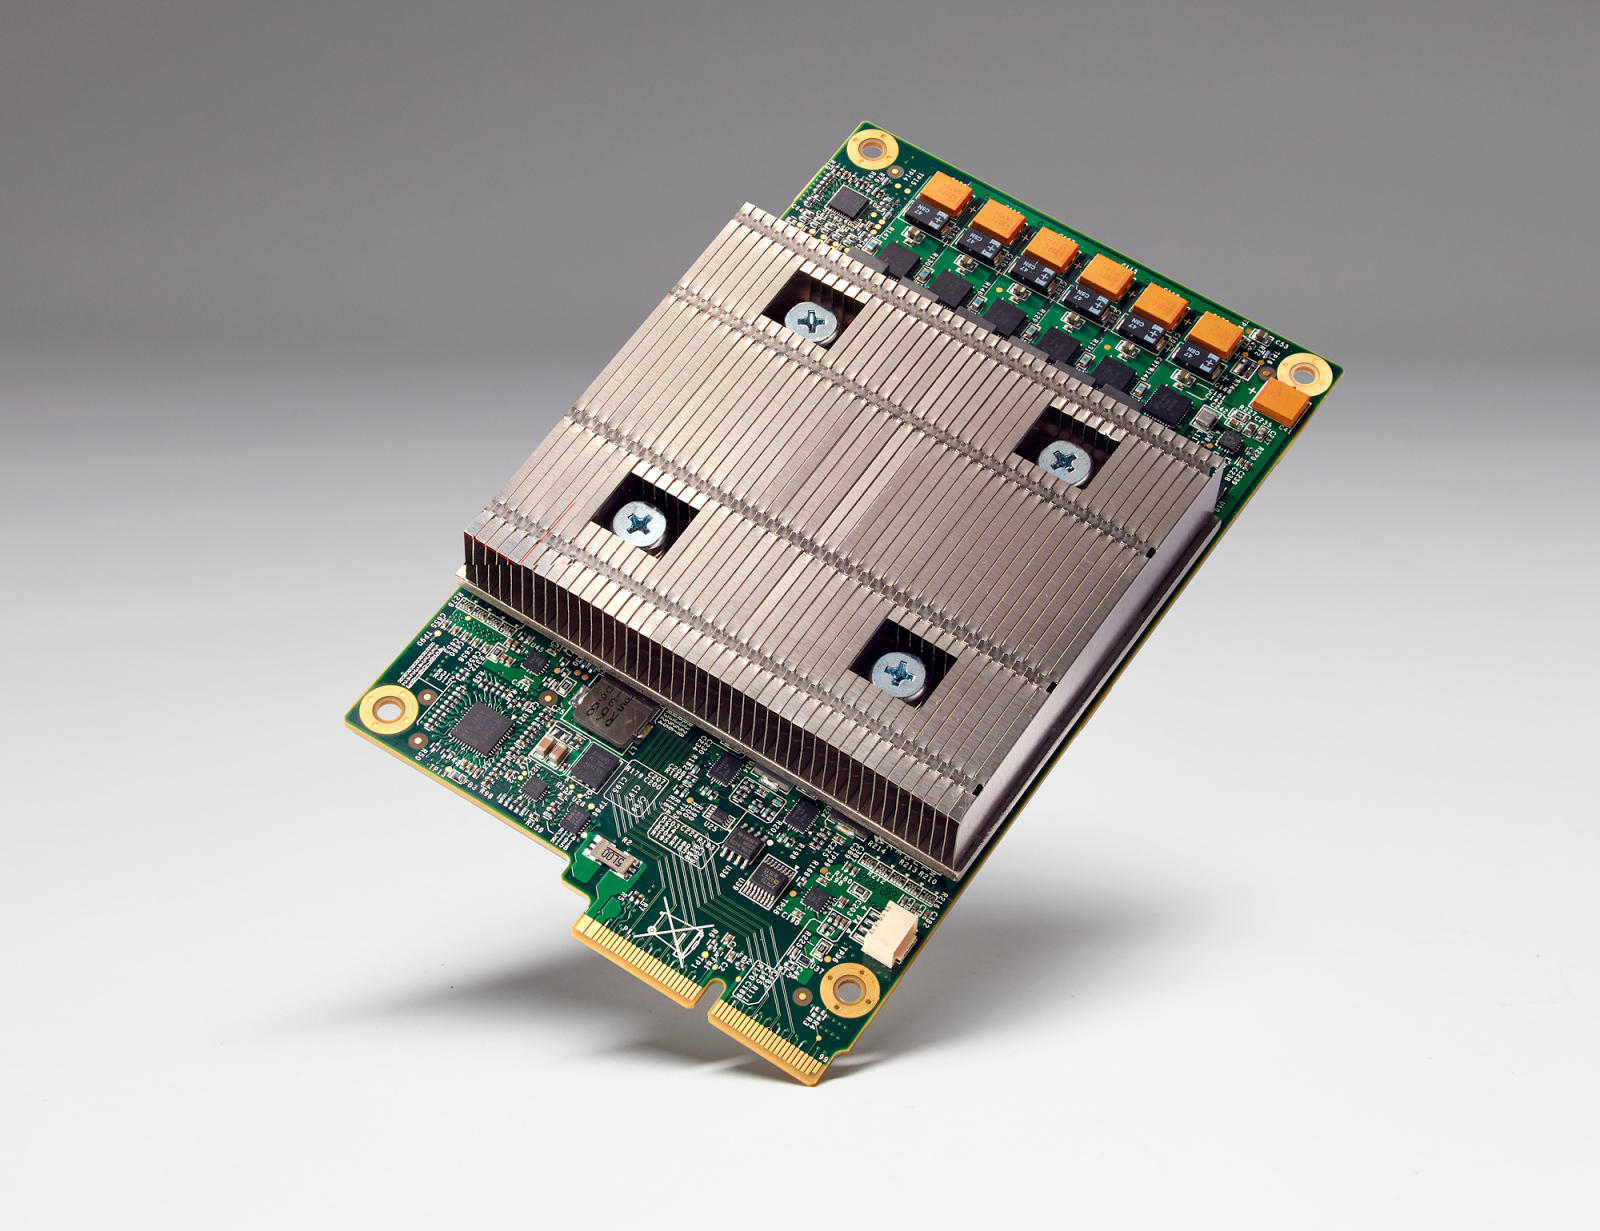
\includegraphics[scale=0.1]{tpu}};
        \draw [white, rounded corners=5pt, line width=5pt]
            (pic.north west) --
            (pic.north east) --
            (pic.south east) --
            (pic.south west) -- cycle;
        \draw (pic)+(0, -2.5) node {\textbf{TPU}};
      \end{tikzpicture}
    \end{column}
    \begin{column}{0.5\textwidth}
      \begin{itemize}
        \item \textit{Coprocessor}
        \item 92 TOPS for 8-bit int
        \item 42 TFLOPS (TPU2)
        \item 24 MB Memory
      \end{itemize}
    \end{column}
  \end{columns}
\end{slide}

\begin{slide}{Hardware: IPU}
  \begin{tikzpicture}[]
    \tikzset{mem/.style={%
      draw, fill=Red, rectangle, text width=0.3mm, text height=2.25mm}}
    \tikzset{proc/.style={%
      draw, fill=Goldenrod, circle, inner sep=1.2mm}}
    \foreach \a in {0, 10, ..., 360} {
      % Memory
      \path (0, 0)+(\a:2.3cm)
            coordinate [mem, rotate={\a+90}] (m\a)
            node [rotate={\a-90}] {\tiny\textbf{M}};

      % Processor
      \onslide<1>{
        \path (0, 0)+(\a:2.9cm) coordinate [proc] (p\a)
              node [rotate={\a-90}] {\tiny\textbf{P}};
      }
      \onslide<2>{
        \path (0, 0)+(\a:2.9cm) coordinate [proc, fill=white] (p\a)
              node [rotate={\a-90}] {\tiny\textbf{P}};
      }

      % Exchange
      \onslide<1>{
        \draw [semithick] (0, 0)
              circle [radius=1.65cm] node [black] {Compute};
      }
      \onslide<2>{
        \fill [llvmblue, semithick] (0, 0)
              circle [radius=1.65cm] node [white] {Communication};
      }

      % P - M
      \draw (p\a) -- (m\a);

      % M - Exchange
      \draw [stealth-stealth, shorten >=0.5pt, shorten <=0.5pt]
            (m\a) -- ++(\a:-0.65cm);

      \node at (0, -3.7) {\textbf{Bulk Synchronous Parallelism}};
    }
  \end{tikzpicture}
\end{slide}

\begin{slide}{Hardware: IPU}
  \begin{columns}
    \begin{column}{0.5\textwidth}
        \begin{itemize}
          \item Startup from Bristol (UK)
          \item Graphcore Colossus
          \item TBR later this year
          \item 1000 Processors/Chip
          \item Mixed Precision Arithmetic
          \item No DRAM
          \item ``Thrives on Sparsity''
        \end{itemize}
    \end{column}
    \begin{column}{0.5\textwidth}
      \centering
      \begin{tikzpicture}
        \node [inner sep=0] (pic) at (0, 0)
              {
\includegraphics[scale=0.25]{graphcore}};
        \draw [white, rounded corners=5pt, line width=5pt]
            (pic.north west) --
            (pic.north east) --
            (pic.south east) --
            (pic.south west) -- cycle;
        \draw (pic)+(0, -2.7) node {\textbf{Graphcore}};
      \end{tikzpicture}
    \end{column}
  \end{columns}
\end{slide}
